%-----------------------------------------------------------------------------
%
%               Template for sigplanconf LaTeX Class
%
% Name:         sigplanconf-template.tex
%
% Purpose:      A template for sigplanconf.cls, which is a LaTeX 2e class
%               file for SIGPLAN conference proceedings.
%
% Guide:        Refer to "Author's Guide to the ACM SIGPLAN Class,"
%               sigplanconf-guide.pdf
%
% Author:       Paul C. Anagnostopoulos
%               Windfall Software
%               978 371-2316
%               paul@windfall.com
%
% Created:      15 February 2005
%
%-----------------------------------------------------------------------------


\documentclass{sigplanconf}

% The following \documentclass options may be useful:

% preprint      Remove this option only once the paper is in final form.
% 10pt          To set in 10-point type instead of 9-point.
% 11pt          To set in 11-point type instead of 9-point.
% authoryear    To obtain author/year citation style instead of numeric.

\usepackage{amsmath}
\usepackage{graphicx}
\usepackage{listings}
\usepackage{url}
\usepackage{color}
%\usepackage{fixltx2e}

\graphicspath{ {images/} }

\begin{document}

\special{papersize=8.5in,11in}
\setlength{\pdfpageheight}{\paperheight}
\setlength{\pdfpagewidth}{\paperwidth}

\conferenceinfo{Design and Implementation of Modern Programming Languages}{December 1--8, 2014, Darmstadt, Hessen, Germany} 
\copyrightyear{2014} 
\copyrightdata%{978-1-nnnn-nnnn-n/yy/mm} 
\doi%{nnnnnnn.nnnnnnn}

% Uncomment one of the following two, if you are not going for the 
% traditional copyright transfer agreement.

%\exclusivelicense                % ACM gets exclusive license to publish, 
                                  % you retain copyright

%\permissiontopublish             % ACM gets nonexclusive license to publish
                                  % (paid open-access papers, 
                                  % short abstracts)

\titlebanner{}        % These are ignored unless
\preprintfooter{}   % 'preprint' option specified.

\title{Reactive Programming in a Distributed Setting}
\subtitle{}

\authorinfo{Iva Toteva}
           {Technical University Darmstadt}
           {iva.toteva@stud.tu-darmstadt.de}
\authorinfo{Nikola Aleksandrov}
           {Technical University Darmstadt}
           {naleks@kom.tu-darmstadt.de}

\maketitle

\begin{abstract}
Distributed programming introduces new challenges for the development of robust and performant data-driven applications. This stems from the fact that changes to values in one part of the application have to be correctly propagated not only within the same device, but also between remote hosts. The tasks becomes even more difficult if the program requires handling dynamic connecting and disconnecting of hosts.

Reactive programming has already proven its benefits in local settings\cite{bridging}. This paper will focus on the ways it can be used to address the afore-mentioned difficulties of distributed programming by examining several studies on Scala libraries, publish/subscribe middleware and concrete algorithms like DREAM, a distributed version of ELM, and SID-UP.

\end{abstract}

% \category{CR-number}{subcategory}{third-level}
\category{C.2.4}{Computer Communication Networks}{Distributed applications}
\category{D.3.3}{Programming Languages}{Language Constructs and Features}

% general terms are not compulsory anymore, 
% you may leave them out
% \terms
% term1, term2

\keywords
Distributed Systems, Observer Pattern, Event-Driven Programming, Reactive Programming, Dependency Graph, Glitches, Consistency Guarantees, Glitch Freedom, Dynamic Networks

\section{Introduction}

Technology has become a part of our everyday life due to the many improvements it brings to our lives. Applications range from large client-server architectures backing up the work of large corporations, through mobile devices used ubiquitously for tracking and sharing sport and social activities, to pervasive computing implementing monitoring and controlling of the ambient. The numerous usages require more complicated networking and architectures to support them. This is where distributed applications come in handy with their resource sharing capabilities, good cost/performance ratio and fault tolerance.

Despite their many advantages, distributed systems also pose some challenges to developers, the most important of which being the correct synchronization between distributed nodes. Exchanging messages from one host to another and upholding different consistency guarantees in particular become much more difficult with the introduction of distribution. Moreover, the task of handling the communication efficiently in a decentralized and potentially dynamic network calls for a revision of the existing paradigms. 

Several solutions have been proposed in order to establish a mechanism that deals with the communication reliably, allowing the establishment and adherence to guarantees regarding the way the messages are passed. We will discuss and compare some of them in terms of their possible applications in dynamic distributed applications. The focus will be on the ways of achieving reactivity of a program. In the current paper we will examine several reactive suggestions and the manner in which they can address the challenges of distributed computing.

This paper makes the following contributions:

\begin{itemize} \itemsep1pt \parskip0pt \parsep0pt
  \item It describes a common organization of a distributed system, such as the publish/subscribe 
  \item It summarizes the main approaches for developing reactive applications in a distributed setting
  \item It outlines the challenges of the development of distributed applications
  \item It introduces the main concepts of reactive programming
  \item Represents a structured analysis of the latest and most exhaustive research papers in the sphere of distributed reactive applications
  \item It argues that reactive programming can be leveraged to address the needs of distributed applications.
\end{itemize}

The rest of the paper is structured as follows: Section 2 summarizes the traditional approaches for ensuring the reactivity of a program. It also describes the organization of general publish/subscribe systems such as JMS. Section 3 introduces the basics of reactive programming as an alternative to these approaches. It also presents the algorithms that will be later compared in terms of the solutions they propose to the common challenges of distributed reactive programming. Section 4 discusses common problems - propagation of changes in reactive applications, ensuring glitch-freedom and handling dynamic network topologies. In Section 5 we give some overview of Related Work. Section 6 concludes the paper, giving a summary of the present study.

\section{Traditional Ways of Ensuring Reactivity}

The term “reactive” stands for responsive, resilient, elastic message-driven systems, as stated by the Reactive Manifesto \cite{rm}. Different solutions have been used in the past in order to ensure the correct message exchange while retaining loose coupling, isolation and location transparency. The most common solutions in the object-oriented setting are the Observer pattern (used as a stand-alone solution or in a publish/subscribe system), Event-driven systems and callback mechanisms, and data bindings.

\subsection{Observer Pattern}

\begin{figure}
\centering
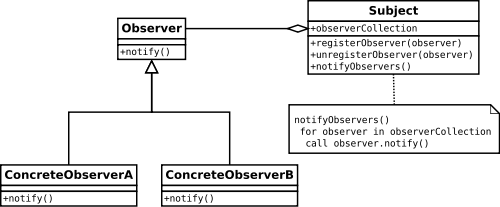
\includegraphics[width=\columnwidth]{observer}
\caption{Observer Pattern}
\end{figure}

The Observer pattern \cite{ojpg} is commonly used to implement distributed event handling. However, the pattern is also highly criticized due to the overhead it creates in terms of boilerplate code that has to be added to the application. Its implementation also involves pollution of the interface of the classes because of the methods added in order to handle the message passing. In addition, it causes inversion of control and can potentially cause memory leaks. The Observer pattern is briefly described by the UML diagram in Figure 1.

Listing 1 shows an example implementation in Scala that implements the following scenario: let us assume that we have three different variables  \textit{a}, \textit{b}, \textit{c} and we want to define a constraint on \textit{c} to be equal to the sum of the other two variables \textit{a} and \textit{b} at all times.

\begin{lstlisting}[frame=single,caption=Observer Pattern in Scala, captionpos=b,linewidth=\columnwidth, language=java, basicstyle=\small, morekeywords={def,val,var,object, trait}, keywordstyle=\color{blue},
numbers=left, numbersep=5pt] 
trait Observable {
  val observers = 
    scala.collection.mutable.Set[Observer]()
  def registerObserver(o: Observer) = {
	 observers += o 
   }
  def unregisterObserver(o: Observer) = { 
	observers -= o 
   }
  def notifyObservers(a: Int, b: Int) = {
	observers.foreach(_.notify(a, b)) 
   }
}

trait Observer {
  def notify(a: Int, b: Int)
}

class Sources extends Observable {
  var a = 1
  var b = 2
}

class Constraint(a: Int, b: Int) 
	extends Observer {
  var c = a + b
  def notify(a: Int, b: Int) = { c = a + b }
}

object Observering {
  def main(args: Array[String]): Unit = {
    val s = new Sources()
    val c = new Constraint(s.a, s.b)
    s.registerObserver(c)
    s.a = 4
    s.notifyObservers(s.a, s.b)
    s.b = 8
    s.notifyObservers(s.a, s.b)
  }
}

\end{lstlisting}

As can be seen from the code, there is a lot of code dealing with the wiring and communication explicitly, thus making the code of the program less readable. Furthermore, in this implementation the changes to the variables are treated in a way that does not let the variable \textit{c} determine which of the two source variables caused the change. In addition, if we have a more complicated program, the code for the updating of \textit{c} will be mixed in with the implementation of the business logic of the application. The implementation of the notification logic also normally adds methods for registering and unregistering observers, which pollute the API of the classes.

\subsection{Events, Callbacks and Data Binding}

The most popular alternatives to the Observer pattern in recent years are events and callbacks. 
Events are easier to use in comparison to implementing the Observer pattern, but also have a couple of drawbacks. For example, in the case of multiple handlers of the same event (which is often the case), all subscribers have to listen for the same event. When the subscribers want to implement the same logic at the occurrence of the event, the code that does the specific goal has to be duplicated on every client and can be considered a violation of the DRY \textit{(Don't repeat yourself)} principle. We will see later in the paper how reactive programming avoids this problem.

Furthermore, there is no way to determine in what order the event handlers will be executed and to determine statically the control flow of the application.

The same statement holds true for callbacks - every subscriber would have to contact the host emitting the messages and pass a reference to the callback function. Callbacks also hinder the static reasoning about the behavior of a program because of the inversion of control.

Microsoft's .NET framework \cite{net} offers an interesting and quite useful approach for propagating data changes in the back-end of the program, in the UI, or between the back-end computations and the UI \cite{dp}. They introduce a special type of properties called ``dependency properties'', which can be defined on objects inheriting from DependencyObject. Basically, if you want to track automatically the changes of a property, a common approach would be to implement it as a DependencyProperty of a specific DependencyObject. 

Each dependency property has to be specially registered using a factory method, so that the framework knows to treat it differently. When this method is invoked, it is passed the following parameters: name of the property, its type, its owner class, default value and a callback that is to be executed when the value of the property changes. Listing 2 shows an implementation of the \textit{\textbf{c = a + b}} example using dependency properties in the C\# programming language. As can be seen in the code listing, we have an object DependencyObjectSum with dependency properties \textit{AProperty},\textit{ BProperty} and \textit{CProperty}, wrapping regular properties \textit{A}, \textit{B} and \textit{C}. When the values of \textit{A} and \textit{B} change, a callback is fired to reevaluate \textit{C}. 

The approach is also widely used with Microsoft's frameworks Windows Presentation Foundation (WPF) and Silvelright. Dependency objects and properties also enable data-binding between controls in the UI and the values in the back-end. For example, we can easily define a page with TextBox controls, which show the values of the \textit{A}, \textit{B} and \textit{C} properties of a DependencyObjectSum object. When the user changes the text in the text boxes which have their Text property data bound to \textit{A} and \textit{B}, the value in the other text box will be automatically reevaluated and changed to the new sum. The code that does that can be seen in Listing 3. 

However, this approach has a couple of setbacks. First, it requires a lot of boilerplate code even in this simple scenario. Second, the wiring requires typing the name of the property as a string, not making use of static type-checking. Thus, a small typo can take hours to debug. Last, dependency objects and properties usually cause a lot of memory consumption overhead, can lead to performance issues and even memory leaks when not handled carefully.

\begin{lstlisting}[frame=single, caption={DependencyObjectSum.cs. In that file are defined three dependency properties, where C changes every time when new values are assigned to A or B} ,captionpos=b,linewidth=\columnwidth, basicstyle=\small, language=java, morekeywords={readonly, set, get, typeof}, keywordstyle=\color{blue}, numbers=left, numbersep=5pt]
 public class DependencyObjectSum : 
		DependencyObject {
  public int A {
   get {
    return (int)this.GetValue(AProperty);
   }
   set {
    this.SetValue(BProperty, value);
    }
  }
 public int B {
   get {
    return (int)this.GetValue(BProperty);
   }
   set {
    this.SetValue(BProperty, value);
   }
  }
 public int C {
  get {
   return (int)this.GetValue(CProperty);
  }
  set {
   this.SetValue(CProperty, value);
   }
  }

public static readonly DependencyProperty
 AProperty = DependencyProperty.Register("A",
 typeof(int), typeof(DependencyObjectSum),
 new PropertyMetadata(0,
 new PropertyChangedCallback(OnAddendChanged)
));

public static readonly DependencyProperty
 BProperty = DependencyProperty.Register("B",
 typeof(int), typeof(DependencyObjectSum),
 new PropertyMetadata(0,
 new PropertyChangedCallback(OnAddendChanged)
));

public static readonly DependencyProperty
 CProperty = DependencyProperty.Register("C",
 typeof(int), typeof(DependencyObjectSum),
 new PropertyMetadata(0, null));

 private static void OnAddedChanged(
   DependencyObject d, 
   DependencyPropertyChangedEventArgs e)
 {
   DependencyObjectSum thisObject = 
    d as DependencyObjectSum;

   if (thisObject != null)
   {
     thisObject.C = 
       thisObject.A + thisObject.B;
   }
 }
}
\end{lstlisting}

\subsection{Publish/Subscribe Middleware}

Publish/subscribe or pub/sub paradigm is a very popular model for designing infrastructure for connecting different systems in a distributed environment.

\bigskip

\begin{lstlisting}[frame=single, caption={DependencyObjectSum.xaml. Here three different text boxes are defined for testing the code from the previous listing},captionpos=b,linewidth=\columnwidth, basicstyle=\small, morekeywords={Source, Path}, keywordstyle=\color{blue},
numbers=left, numbersep=5pt]
 <Grid.Resources>
   <local:DependencyObjectSum x:Key="sum" />
 </Grid.Resources>

 <TextBox Text="{Binding 
	Source = {StaticResource sum}, 
	Path = A, Mode = TwoWay}" />
 <TextBox Text="{Binding 
	Source = {StaticResource sum}, 
	Path = B, Mode = TwoWay}" />
 <TextBox Text="{Binding 
	Source = {StaticResource sum}, 
	Path = C, Mode = OneWay}" />

\end{lstlisting}

 This is so because it can be applied in a  A pub/sub system consists of publishers, subscribers, and a message mediator in between called event service or event brokers. The task of those brokers is to take care of the network that connects publishers and subscribers and to assure that the messages exchanged are going to reach their destination with satisfying performance \cite{pubsub1}. According to  Eugster et al. \cite{pubsub4} the event broker known also as event service is responsible for:

\begin{itemize} \itemsep1pt \parskip0pt \parsep0pt
  \item \textbf{space decoupling} - different participants do not know of each other, but communication between them is possible
  \item \textbf{time decoupling} - publishers and subscribers are not required to be connected to the system at the same time, messages can be exchanged between them even when one is not online
  \item \textbf{synchronization decoupling} - different publishers can create information at the same time, while subscribers consume the events asynchronously.
\end{itemize}

Publishers and subscribers are only responsible for generating and consuming events and all the infrastructure requirements are left for the event service, that is why publish/subscribe systems are very suitable for a distributed setting.

Publishers create information events and put them into the system, while subscribers wait for specific events and consume the generated information. Pub/sub based systems achieve loose coupling because publishers and subscribers do not know anything about each other and the only thing that connects them are the subscriptions and advertisements exchanged in the system.

There are two main types of pub/sub systems - \textbf{subject-}, \textbf{topic-} and \textbf{content based}. The first type defines different subjects or topics. All of the subscribers registered for a topic receive all of the events for that subject, although not all of them might be interested in everything generated for the same topic. That is why another kind of pub/sub systems was introduced - the so-called content-based type. It is considered to be more flexible because subscribers can filter the events generated for a topic based on the content of the message, and handle only those that they are really interested in. Some of the advantages of content-based over topic-based is that it is required to define less subjects and also has less overhead in maintenance \cite{pubsuburl}.

On the other hand implementing content-based publish-subscribe system is not a trivial task. Efficiently matching an event when there are multiple number of subscribers and only one event broker, or efficiently multicasting events when there are many brokers, seems to be an arduous problem especially when the system is geographically distributed and scalability is required. Banavar et al. \cite{pubsub1} contribute by providing a link-matching algorithm that can be used for content-based pub/sub systems to solve the problems mentioned.

Fiege et al. \cite{pubsub2}, Cugola et al. \cite{pubsub3} and Souto et al. \cite{pubsub5} present pub/sub based middleware that has been successfully used in a distributed environment consisting of mobile and wireless devices. Requirements and limitations of such networks are first introduced and then suggestions are given how pub/sub based middleware can help in solving related problems.

Publish/subscribe systems have found an application in mobile sensor networks. They cover the requirement that many participants can generate or consume information, and all nodes in the network should be able to reach the rest. However, in contrast to traditional publish-subscribe systems where nodes are statically situated, mobile devices can change location often and introduce a new topology of the network. Therefore new publish-subscribe based middleware has to be implemented for the scenario where mobile and wireless sensors are used that deals with the typical problems of mobile networks with roaming nodes.

According to the authors of the papers above, middleware based on publish-subscribe paradigm is an appropriate approach for implementing distributed mobile and wireless sensor network system because it provides flexibility, scalability and good performance. However:

\begin{itemize} \itemsep1pt \parskip0pt \parsep0pt
  \item Its implementation usually relies on a variant of the Observer pattern, thus involving inversion of control flow.
  \item A way to deal with roaming publishers/subscribers has to be devised and implemented.
  \item Push based communication from the server to the clients may yield unbounded one-to-many communication.
\end{itemize}
We will now look more closely into a particular publish/subscribe message service - \textbf{JMS}.

\section*{Java Message Service}

\smallskip
JMS that stands for Java Message Service is a messaging standard used in Java EE platform for creating, sending, receiving and reading information messages between different client programs \cite{jms} \cite{jmsd}. This technology is applicable in a distributed environment and offers loose coupling, reliability and asynchronous communication.

Before giving detailed information about JMS let us first briefly introduce the general idea of messaging that is used today. Current distributed systems consist of numerous end hosts where different client applications establish connections and communicate with each other. In order to achieve reliable communication and satisfying speed with very short delay, stable infrastructure has to be built for such an environment.

The messaging concept is the technology that offers exchange of information between multiple, potentially different software components and applications, by preserving the already mentioned requirements. It offers an intermediate agent that handles the distribution of messages and takes care that they reach their destination. The main idea is to build an infrastructure, where different software programs can communicate with each other, without explicitly knowing much about each other. What matters is that when a message is generated from a client, it is sent to other clients that are interested. If the data format of the message is unknown for some of the clients, the intermediate agent takes care of the translation and maintenance of the environment, so that all client applications can understand each other.

As mentioned before, JMS API is an important component from the Java Enterprise Edition platform and was built for solving communication problems between different technologies that are also part of Java EE.
	
Every JMS application consists of the following parts:

\begin{itemize} \itemsep1pt \parskip0pt \parsep0pt

\item \textbf{JMS provider} - a Java implementation of message oriented middleware that offers features for administration and control
\item \textbf{JMS client} - an application written in Java that can produce and consume messages. Clients are divided into two categories: \textbf{JMS publisher/producer} and \textbf{JMS subscriber/consumer} depending on the action that they perform. It is also possible that a client can be both a producer and a consumer in the same distributed environment.
\item \textbf{JMS message} - wraps the object that is used for transferring the information between different JMS clients.
\item \textbf{JMS queue} - a mechanism that assures that every consumer will receive the message no matter if it is interested or not. JMS queue is different from the normal queue that assures delivering of items at the same order as they entered the queue. JMS queue takes care that the consumer receives the message only once, but does not provide any guarantees as to the order in which the messages will be consumed by the subscribers.
\item \textbf{JMS topic} - a way to distinguish between different messages. Consumers register for specific topics and  filtering is performed to ensure that only interested subscribers will be notified of a published message.

\end{itemize}

Another important feature of JMS is the programming model. There are two different implementations:

\begin{itemize} \itemsep1pt \parskip0pt \parsep0pt
\item \textbf{Point-to-point} - This programming model consists of a message sender, a consumer and a queue that connects them. For every consumer there is one message queue that assures that the message will be delivered. Every message stays in the queue until a consumer receives it and sends an acknowledgment for it or it expires. It is not required that both the producer and the consumer should be online upon sending or consuming the message. If there is no registered consumer for a message queue, all messages remain inside the queue until a consumer asks for them. Advantage of this programming model is that messages are always delivered to consumers and no data is lost. On the other hand in some applications consumers might not be interested in all type of messages, that is why another programming model is used where consumers can subscribe for specific messages – publish/subscribe.
\item \textbf{Publish/subscribe} - JMS implements all features for publish/subscribe model that has already been discussed earlier in the paper. It is worth mentioning that in addition, the JMS API offers the use of durable subscriptions – messages are sent even when the subscribers are not active.

\end{itemize}

When a message is either sent or received, it is very important for JMS API to distinguish between two message consumptions:
\begin{itemize} \itemsep1pt \parskip0pt \parsep0pt
\item \textbf{Synchronous} - when receive method is called, the execution thread of the consumer is blocked until the message is received or it times out.
\item \textbf{Asynchronous} - the client can register a message listener with a consumer. When a message reaches its destination, that listener calls the specific method that handles the message. In this way the execution thread is not blocked and the consumer can perform other tasks, while still reading the message.

\end{itemize}

We are not going into technical details how JMS is used for building applications, as that falls outside of the scope of this paper. We refer to JMS API as another solution for communication between numerous end hosts in the same distributed environment.

\section{Reactive Programming}

Reactive programming aims to render problems of communicating information between nodes obsolete by introducing a new concept of message propagation. It offers immediate change of defined variables during the execution of the program without explicit need for reassignment of the new value.

Let us refer to the example used in Section 2.2 in order to illustrate one significant feature of reactive programming. We have defined variables \textit{a}, \textit{b} and \textit{c}, where \textit{c}  is dependent on two others variables --  \textit{a} and \textit{b}. If \textit{a} and \textit{b} receive new values, but \textit{c} is reevaluated only with the new value of \textit{a} and with the old value of \textit{b}, or in other words a partial update for \textit{c} has occurred, resulting in a meaningless value of the variable \textit{c}. Variable \textit{c} should reevaluate only after both \textit{a} and \textit{b} have their new values.
In REScala the example from above could be implemented as in Listing 4.

\begin{lstlisting}[frame=single,caption={Reactive Sum},captionpos=b,linewidth=\columnwidth, basicstyle=\small, language=java, morekeywords={val, Signal}, keywordstyle=\color{blue}]
	val a = Var(1)
	val b = Var(2)
	val c = Signal { a() + b() }
\end{lstlisting}

The types used in the example are built-in the REScala framework and are used to define reactive values.

\begin{itemize} \itemsep1pt \parskip0pt \parsep0pt
  \item \textbf{Vars} are used to represent atomic types, such as int, string, etc., and can be used in reactive expressions (signals).
  \item \textbf{Signals} are declared as a constraint expression and their values can change automatically over time when other variables in the expression change. That is why sometimes in the literature signals are also referred to as \textbf{Behaviors}. It is possible for a signal to depend on another signal. 
  \item \textbf{Reactives} - a common term for vars and signals to describe the concept of time-changing values, that are introduced in "Towards Reactive Programming for Object-Oriented Applications" \cite{towards} . When the respective observable and reactive variables that participate in the same reactive expression are spread across different hosts we refer to them as \textbf{remote reactives}.

\end{itemize}

There are two important concepts that reactive programming deals with -- \textbf{data flow} of the program and \textbf{propagation of changes}.

The data flow concerns the passage of information in the form of data and messages from one part of the application to another. In reactive programming, the focus is not so much on method calls (as is the case with Object-Oriented programming), but on the logically existing dependencies between variables. These dependencies are usually depicted using a directed graph, where the nodes represent the variables of the program and the edges - the dependencies between them. The dependency graph for our simple example is shown in Figure 2.

\begin{figure}
\centering
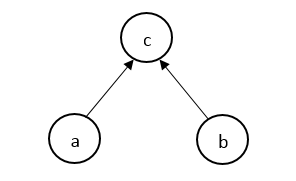
\includegraphics[width=4cm]{dependencyGraph}
\caption{Dependency Graph}
\end{figure}

This \textbf{Dependency Graph} is formally defined as a directed graph \textit{D = \{V, E\}}, where \textit{V} are all variables V = $v_{1}$,$ v_{2}$, ... , $v_{n}$  are  defined in a component of a reactive program, and \textit{E} represents all the edges in the graph. There is an edge $e_{ij}$ from variable $v_{ i}$ to variable $v_{j}$ , if  $v_{j}$ is a reactive variable defined through an expression in which $v_{i}$ participates.  We also say that a variable $v_{c}$ is dependent on a variables $v_{a}$ or $v_{b}$ if there are paths from $v_{a}$ or $v_{b}$ to $v_{c}$ \cite{dream}.

In general, the lifecycle of reactive applications is described in terms of update turns.  An \textbf{update turn} starts when a change occurs inside the reactive network of an application and this change has to be passed on to the dependent variables and cause their revaluation. These update turns can be split into the following phases: \textbf{admission phase} and \textbf{propagation phase}. The admission phase is the first one and it is characterized by the fact that new values for some input nodes are assigned. After that the propagation phase starts, during which the new values of the changed nodes are made visible to the variables that use them. Only the nodes that are transitively reachable from the source nodes have to participate in the propagation phase, because only dependent reactive values have the potential to be updated \cite{sidup}. Different solutions have been proposed in order to ensure that the changes will be correctly propagated in the dependency graph with different consistency guarantees.

The main issues with the propagation of changes is determining a way in which all dependent nodes are evaluated with least amount of messages passed and without obtaining spurious values. Such inconsistencies may be obtained as a result of a partial update for example -- when the value of a variable is overwritten without taking into account the new values of all the variables it depends on. The term that is used to denote such invalid states of a variable or state of the programs is \textbf{glitches}.

In a local setting, glitches can be avoided by topologically sorting the variables and updating them in levels. In this way, a variable is only updated after all its dependent variables have changed their values. In our example the variables \textit{a} and \textit{b} can be considered at level 0, while \textit{c} is at level 1. Therefore, \textit{a} and \textit{b} can be potentially evaluated and update at the same time and the evaluation of \textit{c} can occur only after that. In that way \textbf{glitch freedom} can be achieved.

Another thing that reactive applications usually consider is \textbf{dynamic dependencies}. In a reactive program it is possible that at some point reactive variables change the variables on which they depend, as compared to other stages of the application. This must be properly reflected in the dependency graph in order to propagate the changes correctly. Dynamic dependencies provide the following two important features \cite{sidup}:

\begin{itemize} 
\item\textbf{Conditionally accessed input values} - This feature describes the case when a variable is dependent on other variables, but not always on all of them. If at the current point of execution our main variable is not dependent on the updated input value, a reevaluation is not needed.

For instance, if we have \textit{z = if c then x else y, z} will always depend on the value of \textit{c}. However, depending whether \textit{c = true} or \textit{c = false, z} will need to be evaluated either when \textit{x} changes or when \textit{y} changes. We say that \textit{z} has a dynamic dependency on \textit{x and y}.

\item\textbf{Higher Order Reactives} -– These are reactive values that depend on other reactive values. That feature is very important in a distributed setting, because it allows dynamic dependencies. In a distributed environment where hosts can connect and disconnect at any time, higher order reactives are needed to ensure the proper functioning of the system \cite{sidup}.

\end{itemize}

Reactive languages also support the typical for the imperative style of programming events. For example, in REScala \cite{rescala} there is built-in event notifying when a change to a reactive value has been made. There are also a lot of conversion functions that create signals from events.

In a nutshell, reactive programming keeps the expressiveness of imperative languages, but also introduces new easier ways of handling message propagation. In solves the problems connected to the use of the Observer pattern: \textit{verbosity, lack of static reasoning, inversion of control}. It manages the dependencies between values in the language implementation, not in the application logic, thus achieving better separation of concerns. There is also no scattered duplicated code, as is the case when events or callbacks are used and the developer is freed from the need to “manually” update the application layer with the changes arisen elsewhere in the program.

We will investigate some of the proposed solutions for reactive message propagation in terms of the way they implement the monitoring of the connected peers and carry out the communication between them.

\subsection{Local Reactive Programming}
\subsubsection{Scala.React and Scala.Rx}

Scala.React and Scala.Rx are two libraries built on top of Scala that address the need for reactive programming in the local setting. Both libraries use topological sorting with priority queue to order the nodes according to their dependencies. Scala.React uses only one thread and thus only one node is updated at a time. The default behavior of Scala.Rx is the same, however it also allows a parallel propagator to be used instead of the default sequential one. In this way, variables from one layer can be removed from the queue and processed at the same time concurrently. 

Neither of the two libraries however has been used in a distributed setting upholding change propagation guarantees. We will later look into a distributed update algorithm for REScala that manages to do that.

\subsubsection{ELM}
The ELM algorithm proposed in \cite{elm} suggests an algorithm for propagating value changes in a local setting. The authors suggest a network organization which includes a central coordinator. This component's job is to broadcast every update turn's start to all input nodes. Every node then sends a “change” or “no change” pulse depending on whether it has been changed or not in this update turn. When a node receives signals from all nodes that it has a dependency on in the current turn, it reevaluates its value and sends a signal itself. The evaluation finishes when all nodes send a signal with their state.

The algorithm supports pipelining, i.e. the pulses can be propagated in wave fronts, thus enhancing parallelism in the propagation phase, from which distributed settings can benefit.

Drechsler et al. \cite{sidup} devise a variation of this algorithm named ELM\textsuperscript{s} which can be used in distributed programming.

\subsection{Distributed Reactive Programming}

\subsubsection{DREAM}
DREAM \cite{dream} is a distributed reactive middleware implemented in Java. It defines an abstract Observable class, which can be inherited from in order to create different specific observable types, such as \textit{ObservableInteger or ObservableString} and create specific instances of these classes \textit{(ObservableInteger(1) or ObservableInteger(5) and so on)}. Every method of an observable class that returns a non-void result is called an observable method. These methods can return reactive objects. In that case, the methods that manipulate the returned reactive objects are annotated using Java annotations, so that the framework knows that after the execution of these methods, the changes to the reactive objects must be further propagated. 
Reactive objects can also be created from a reactive expression using a factory class. In the introduced notation reactive objects correspond to signals (behaviors).
In DREAM every component has a unique name, which can be used to identify the observable or reactive object. This is done using a discovery naming service, which can search by name, type, component or a combination of these properties.

The architecture of DREAM consists of so-called clients and brokers. The clients are the end hosts that have reactive variables and the brokers are the infrastructure that enables different clients to communicate with each other. Additional a registry can be implemented to be used by brokers to check different information about other brokers and clients. The brokers are the connection between the clients and their logical structure may be thought of as an undirected acyclic network. This means that the network between the different brokers is established based on the cost of the edge in the weighted graph and can be changed at any time. This is done for example when the graph becomes disconnected and brokers are not able to ping each other.

The communication between different clients inside that system is based on the following three basic messages -- \textbf{advertisement}, \textbf{subscription} and \textbf{notification}.
Clients advertise some reactive values and subscribe to changes of other reactive values. If the reactive value that a client declares changes, the client sends notifications to all subscribed reactive values. Those subscribed reactive values can either be located on the same client, or on other hosts. When the subscribed variables are at the same host, the local dependency graph layering takes care of its proper propagation. When the subscription to a notification is on a remote host, the broker takes care for the propagation of changes. Brokers are responsible for detecting depending events and also for notifying the components. The following three characteristics are important for the broker network:

\begin{itemize}
\item all brokers deliver the advertisements
\item components receive subscriptions that fully match their advertisements
\item notifications are sent only to those components that have valid subscription.
\end{itemize}

\subsubsection{SID-UP}
SID-UP \cite{sidup} is an update algorithm for distributed reactive programming. It has been implemented in Distributed REScala to allow the use of the programming language in a distributed setting.

SID-UP also considers two phases of the change propagation of a value. In the admission phase it uses a central coordinator to allow only one update turn at a time. However, the coordinator does not broadcast the update turn's start as in the ELM algorithm. Instead, the nodes that want to initiate an update contact it in order to obtain permission to start updating a source value. In addition, every node stores information about the source nodes it is transitively connected to and dependent upon.

Furthermore, each pulse carries information about all sources changes during the current update turn. This allows only nodes reachable from the changed sources and the edges between them to be involved in the transmitting and waiting for pulses in the propagation phase.

Once the propagation phase starts, the nodes that can be potentially updated wait for pending nodes, on which they depend. After all dependencies have been evaluated, the current node updates its value and sends a pulse further on. The nodes also keep a local mirror copy of the nodes, on which they depend. When the original node changes, it pushes the change to the mirror node, from where the dependent node extracts the changed value in a pull-based manner.

This organization allows all dependent nodes to execute on different threads and be governed only by the pulses they receive.

\subsubsection{AmbientTalk/R}
AmbientTalk \cite{loosely} is an experimental scripting programming language that is designed for the purposes of distributed programming. There is a bridge between AmbientTalk and Java, ensuring that objects of one language can communicate with objects from the other, thus providing good interoperability between the two languages.

AmbientTalks is an event-driven programming language that supports only event loop concurrency. All concurrent activities are represented as events, handled sequentially by an event loop thread. The distributed objects communicate by passing asynchronous messages.

AmbientTalk/R is a reactive extension of AmbientTalk that introduces support for reactive programming. Reactive variables can be defined using the makeReactive method on regular objects. The implementation defines two types of methods – Accessor and Mutator methods. The latter are required to be annotated using a special syntax which ensures that the system must take special care to avoid glitches after the method is executed.

\section{Challenges of Distributed Programming}
Each of the presented solutions addresses the common problems of developing reactive applications in a distributed setting. The major concern is ensuring correct change propagation of the variables taking into account the dependencies between the variables. Another addressed matter is the way these suggestions can handle dynamic changes in the network, which is a frequently observed scenario with distributed environments.

\subsection{Change Propagation Guarantees}
\subsubsection{Scala.React and Scala.Rx}
As Scala.React and Scala.Rx count on topological sorting of the nodes, there must be a centralized coordinator that keeps track of the whole network and manages the communication. In a distributed setting, such a solution is not very practical, as it yields unbounded one-to-many communication. This would not only increase the network traffic, but also render impossible any attempts on performing the computations in parallel. Therefore, in its pure form it is not applicable in a distributed environment.

\subsubsection{Publish/Subscribe Systems}
Zhang et al. \cite{totalorder} propose a different classification of change propagation guarantees. Provided that Dest(m) is the set of subscribers that message m should be delivered to, the following types of total orders are defined:

\begin{itemize} \itemsep1pt \parskip0pt \parsep0pt
  \item \textbf{Per-Publisher Total Order}: For any two messages m and m' and any two processes p and q, where {p, q} $\in$ Dest(m) $\cap$ Dest(m'). If sender(m) = sender(m'), then p delivers m before m' if and only if q delivers m before m'.

  \item \textbf{Local Total Order}: For any two messages m and m' and any two processes p and q, where {p, q} $\subseteq$ Dest(m) = Dest(m'). p delivers m before m' if and only if q delivers m before m'.

  \item \textbf{Pairwise Total Order}: For any two messages m and m' and any two processes p and q. If {p, q} $\subseteq$ Dest(m) and {p, q} $\subseteq$ Dest(m'), then p delivers m before m' if and only if q delivers m before m'.

\end{itemize}

The per-publisher total ordering property can be achieved by enforcing FIFO links between the nodes in the network, e.g. by using TCP as the communication protocol between nodes when there are no cycles in the topology. When there are multiple paths between the nodes in the network, the first message may take a detour and arrive after the second one. Zhang et al.\cite{totalorder} assume an acyclic overlay topology of brokers with FIFO links between brokers, which is sufficient to ensure per-publisher total order.

When it comes to local total order, it can be proven that it can be ensured only if there is knowledge of the subscribers for any given message. In a content-based system, this would require a centralized coordinator that calculates all subscribers for a message and sorts out the order in which they should be propagated.

As for pairwise total order, the authors prove that it can be ensured if there paths between the publishers and the end points include a common broker node. In other words, if the publisher of message m is pub and the publisher of message m' - pub', the receivers of both messages - $s_{1}$ and $s_{2}$, the paths between pub and $s_{1}$ and $s_{2}$ - $Q_{1}$ and $Q_{2}$ and the paths between pub' and $s_{1}$ and $s_{2}$ - $Q_{1}$' and $Q_{2}$' respectively, then $Q_{1}$ $\cap$ $Q_{2}$ $\cap$ $Q_{1}$' $\cap$ $Q_{2}$' $\neq$ $\emptyset$  ensures that the messages will be delivered at both subscribers in the same order. However, when the subscribers do not have a common broker, it is possible that the messages will not be delivered in the same order. For that case the authors choose a solution that involves detecting and resolving conflicts.

The algorithm executes a conflict-detection algorithm on each broker, checking if there are potential conflicts. A conflict would arise if there are two messages which are going to pass through the broker from different source paths and go into different destination paths. If at the time a broker receives a publication p, there is at least one advertisement whose next hop coincides with the next hop of a  is that is the case, the program is redirected to the conflict resolution handling method.

The conflict resolution relies on the transmission of acknowledgments. Each publication is assigned a unique ID - a combination of its publisher's ID and a sequential counter incremented for the specific publisher. If a broker detects possible conflicts, it will add to the publication a request for the next brokers to send an acknowledgment if they can determine that there is no conflict. The message is transmitted along with this request among brokers, but it is handed to a subscriber only after such an acknowledgment is received.

\subsection*{Java Message Service}

As mentioned before, JMS takes advantage of a message queue, but it has different properties than the traditional one. An ordinary queue would take care that all messages from the queue are recieved at the consumers in the same order in which they entered the queue. At the same time, a JMS queue only assures that a message is processed exactly once. That feature of JMS has a significant drawback in the application of reactive programming, because the order of the processed messages  is very important for achieving glitch freedom. That is why we can conclude that Java Message Service is not suitable for implementing reactive applications in distributed setting \cite{jms} \cite{jmsd}.

\subsubsection{AmbientTalk/R}
Carreton et al. \cite{loosely} base their algorithm on a publish/subscribe architecture. The system is implemented in the reactive AmbientTalk/R. It handles reactive value changes using the standard dependency graph stratification approach - the interpreter constructs a dataflow graph from the variables. Then, the updates to the values are scheduled in a single event loop, which suffices to avoid glitches in the local setting. 

When it comes to the distributed setting, the problem of synchronization between the different hosts arises. Now, there is not only one event loop to consider, but a number of them. The solution suggested introduces the concept of ambient behaviors that allow loosely-coupled propagation of changes to remote reactive values based on publish/subscribe. 

To address the needs of distributed ad hoc networks, the authors introduce two new constructs - ambient behaviors, which have a role corresponding to that of publishers in Pub/Sub systems, and ambient references, which are the analog of subscribers. Ambient behaviors are used to create local reactive variables and ``export'' them to the other hosts in the system. By subscribing to these behaviors, dependent nodes ensure that the changes in the variables' values will be propagated to them.

However, as the focus of the research paper is on loosely coupled networks with roaming devices, the authors assume that no information about the network should be included in the implementation, which renders impossible any consistency guarantees and glitch avoidance.

\subsubsection{DREAM}
DREAM \cite{dream} implements three different types of consistency guarantees:

\begin{enumerate}
  \item \textbf{Causal semantics} -- ascertaining that the components receive events that are potentially causally related in the same order in which the events have occurred. For example if an event \textit{A} occurs before an event \textit{B} in the same process, than all the components should first see the result of event \textit{A} and then the result of event \textit{B}. In addition, every write event happens before every update event.  

This is ensured by the use of the TCP point to point protocol between component and broker, as well as between brokers. Due to TCP protocol, messages are delivered exactly once and in the order that they are expected to -- First in first out.

  \item \textbf{Glitch free semantics} -- making sure that no partial updates occur and a reactive value is update only after all its dependencies. 

In order to achieve that guarantee, each broker receives the expression for every  reactive value that is created inside a component. In that way brokers can create a dependency graph of the reactive values, which allows them to propagate changes correctly and identify possible sources of glitches. Furthermore, DREAM first calculates all notifications that a specific component has to receive and only afterwards attaches that information to any of the notifications sent to that component. The difference to the causal semantics is that a notification waits in a queue for all other notifications to be delivered before sending out the new value of the reactive variable.

  \item \textbf{Atomic semantics} -- guaranteed when all messages are received in the order in which they arose. If a couple of changes occur on variables inside a component, all dependent variables should receive the update messages in the way they were produced. Furthermore, when there is a write event (changing a value for a variable v in a component), all directly and indirectly dependent on \textit{v} variables should be updated in a single atomic operation. This ensures both causal and glitch-free semantics.
  
DREAM implements atomic semantics using a Ticket Granting Server. When a broker receives a notification for a change in a variable, the broker contacts the TGS for all the leaves in the dependency graph that are dependent on that change. TGS returns them to the broker and observes if the broker sends the notifications to all of them in the correct order. When TGS receives acknowledgments for every notification it continues with the next request. This type of locking mechanism ascertains that an update request from only one broker can be processed at a time.

\end{enumerate}
\subsubsection{ELM\textsuperscript{s}}
ELM \cite{elm} ensures that glitches are avoided by allowing only one update to be triggered at a time and having every node wait for the incoming dependencies. Messages being passed from every progenitor node to its dependencies, regardless of the fact whether their values have been changed. As every node waits for a pulse from all its dependencies, a partial update cannot occur. 

At the same time, even the revised version of the algorithm may not be practical in a distributed setting, as the large number of messages that have to be passed will generate a lot of network traffic and can increase the bandwidth requirements.

\subsubsection{SID-UP}
SID-UP \cite{sidup} adopts a similar approach to ELM. However, instead of having a centralized coordinator broadcast the update turn to all nodes, the nodes contact the centralized entity when they wish to update a value. The coordinator allows only one update turn to be carried out at a time and allows or denies the requests accordingly. In this way one-to-many unbounded communication is avoided. 

In addition, SID-UP requires passing messages only from nodes actively involved in the update. This is made possible by the fact that every node is aware of the dependencies it has and the pulse carries information of the nodes being updated. In that way, unaffected hosts can be exempt from the message passing, which has the potential to save a lot of network traffic.

\subsection{Dynamic Network Topology}

The different authors suggest different approaches for handling dynamic network topologies.

\subsubsection{Pub/Sub}
The Publish/Subscribe paradigm is developed specifically to implement loose coupling between message providers and consumers. Therefore, it provides good support for dynamic network topology. The authors Zhang et al. \cite{totalorder} specify two reliability guarantees:

\begin{enumerate}
  \item \textbf{Liveness}: If a message m is sent by a process p to its destination group Dest(m), then all processes in Dest(m) will eventually deliver m.
  \item \textbf{Safety}: If messages m and n are delivered to both processes p and q, then m and n are delivered to both p and q in the appropriate order.
\end{enumerate}

The paper proves that it is impossible to withhold both guarantees provided that a failure occurs. A total ordering semantics is classified as "weak" if it ensures safety, but not liveness. The focus of the study is on safety, thus devising their algorithm in a way that it implements weak total ordering semantics. However, the authors also outline an approach that can be followed to implement liveness instead.

\subsubsection{Ambient References and Behaviors}
AmbientTalk/R proposes a new construct that handles the network changes. As the paper targets mobile ad-hoc networks, it does not rely on the standard architecture of Pub/Sub systems, involving a broker mediator. Instead, they define “ambient references” -- an abstraction over the appearing and disappearing services in the network. Basically, these ambient references represent a collection of nearby services of the same type. They are constantly kept up-to-date by the ambient reference itself using autonomous UDP queries.

An ambient reference is created using the ''ambient'' keyword.

When a node wants to multicast a message to all services of a specific type, it sends a message to the ambient reference and the framework makes sure to forward it to all available nodes in the collection.

\subsubsection{DREAM}
DREAM \cite{dream} does not include any mechanisms for handling roaming nodes and as of now does not support dynamic network topologies.

\subsubsection{ELM}
ELM does not originally support dynamic changes in the network and dynamic dependencies. However, the authors of SID-UP \cite{sidup} show that it can be extended to include higher order reactives and consequentially - dynamic dependencies. They develop a mixture of ELM and SID-UP, which they call $ELM^s$, implemented as follows:

\begin{itemize}
\item Global update propagation is introduced by collecting all sources into a centralized coordinator which is responsible for initiating update turns globally
\item The source identifier sets are removed from all nodes and it is ensured that every node will always process every update turn
\end{itemize}

The proposed modified algorithm behaves like the way ELM does when propagating a single turn. It still requires unbounded one-to-many communication in the admission phase and no involvement of the central coordinator in the propagation phase.

However, by gaining support for dynamic dependencies and higher order reactives, it loses the ability to pipeline change propagations.

\subsubsection{SID-UP}
SID-UP \cite{sidup} supports dynamic topology changes in the same way it handles dynamic dependencies among variables in the dependency graph - through higher order reactives. The changes in the network require that the sets of identifier nodes stored on their dependent nodes be updated. First, the nodes which are immediately affected are updated, and then the changes are propagated using the standard propagation algorithm. The nodes keep a flag whether their dependencies on other nodes have changed similarly to their behavior when the value of a variable is updated. When changed, the node forwards the changed or unchanged pulse for the set of dependencies along with the one for the value it keeps.

\section{Related Work}
Reactive programming was first introduced with the aim to support interactive animations in Haskell \cite{haskell}. More recently, Haskell was also extended to include constructs expressing reactive values, corresponding to vals and signals in the notation used in this paper, as well as events \cite{haskell2} \cite{haskell3}. FrTime \cite{scheme} is a reactive language implemented for Scheme, that along with the discussed Scala.React, Scala.Rx and REScala conclude the most important reactive programming technologies in the functional programming world.

As already described, AmbientTalk/R is a reactive programming solution for Java. Flapjax \cite{javascript} for JavaScript and Rx \cite{netrx} for .NET applications conclude the most popular reactive libraries.

Most if not all of these libraries include consistent change propagation using  stratification of the dependency graph in the local setting. However, some of the frameworks are not suitable for use in a distributed environment (e.g. because the language they target cannot be used both on the server and the client), or do not provide any glitch guarantees in that case. 

\section{Conclusions}
In this paper we have shown that reactive applications can be very useful in distributed programming. First, we have started our work by showing the drawbacks that the traditional ways of implementing reactivity have. We have also described the conventional publish/subscribe system organization. Second, we have introduced the reactive programming paradigm and its most important concept.

After we have gathered enough basis knowledge for reactive programming in a distributed setting we compared existing approaches, such as Scala.React, Scala.Rx, ELM, SID-UP, AmbientTalk/R and DREAM. The criteria that we have chosen when conducting the comparison between the different algorithms were the way the systems ensure glitch freedom and achieving satisfying reactivity in the context of joining and leaving hosts. Our study finds Distributed Reactive Programming Middleware (DREAM) and Source Identifier Update Propagation Algorithm (SID-UP) to be the most  thorough and complete papers, shaping out the future path of reactive distributed programming.

%\appendix
%\section{Appendix Title}

%This is the text of the appendix, if you need one.

\acks

This paper has been written for the Seminar Implementation of Modern Programming Languages at Technical University Darmstadt under the supervision of PhD Guido Salvaneschi.

% We recommend abbrvnat bibliography style.

\bibliographystyle{abbrvnat}

% The bibliography should be embedded for final submission.

\begin{thebibliography}{}
\softraggedright

\bibitem{towards} Salvaneschi, Guido, and Mira Mezini. "Towards Reactive Programming for Object-Oriented Applications." {\em Transactions on Aspect-Oriented Software Development XI.} Springer Berlin Heidelberg, 2014. 227-261.

\bibitem{sidup} Drechsler, J., Salvaneschi, G., Mogk, R.,  Mezini, M. (2014, October). Distributed REScala: an update algorithm for distributed reactive programming. {\em  In Proceedings of the 2014 ACM International Conference on Object Oriented Programming Systems Languages and Applications} (pp. 361-376). ACM.

\bibitem{dream} Margara, Alessandro, and Guido Salvaneschi. "We have a DREAM: distributed reactive programming with consistency guarantees." {\em Proceedings of the 8th ACM International Conference on Distributed Event-Based Systems.} ACM, 2014.

\bibitem{bridging} Salvaneschi, Guido, Gerold Hintz, and Mira Mezini. "REScala: Bridging between object-oriented and functional style in reactive applications." {\em Proceedings of the of the 13th international conference on Modularity.} ACM, 2014.

\bibitem{loosely} Carreton, A. L., Mostinckx, S., Van Cutsem, T., and De Meuter, W. (2010). Loosely-coupled distributed reactive programming in mobile ad hoc networks. In {\em Objects, Models, Components, Patterns } (pp. 41-60). Springer Berlin Heidelberg.

\bibitem{multitier} Reynders, Bob, Dominique Devriese, and Frank Piessens. "Multi-tier Functional Reactive Programming for the Web." {\em  Proceedings of the 2014 ACM International Symposium on New Ideas, New Paradigms, and Reflections on Programming and Software.} ACM, 2014.

\bibitem{pubsub1} Banavar, G., Chandra, T., Mukherjee, B., Nagarajarao, J., Strom, R. E., and Sturman, D. C. (1999). An efficient multicast protocol for content-based publish-subscribe systems. In {\em Distributed Computing Systems, 1999. Proceedings. 19th IEEE International Conference} on (pp. 262-272). IEEE.

\bibitem{pubsub2} Fiege, L., Gärtner, F. C., Kasten, O., and Zeidler, A. (2003, June). Supporting mobility in content-based publish/subscribe middleware. In {\em Proceedings of the ACM/IFIP/USENIX 2003 International Conference on Middleware } (pp. 103-122). Springer-Verlag New York, Inc..

\bibitem{pubsub3} Cugola, Gianpaolo, and H. Jacobsen. "Using publish/subscribe middleware for mobile systems." {\em ACM SIGMOBILE Mobile Computing and Communications Review } 6.4 (2002): 25-33.

\bibitem{pubsub4} Eugster, P. T., Felber, P. A., Guerraoui, R., and Kermarrec, A. M. (2003). The many faces of publish/subscribe. {\em ACM Computing Surveys} (CSUR), 35(2), 114-131.

\bibitem{pubsub5} Souto, E., Guimarães, G., Vasconcelos, G., Vieira, M., Rosa, N., Ferraz, C., and Kelner, J. (2006). Mires: a publish/subscribe middleware for sensor networks. {\em Personal and Ubiquitous Computing}, 10(1), 37-44.

\bibitem{totalorder}Zhang, Kaiwen, Vinod Muthusamy, and H-A. Jacobsen. "Total order in content-based publish/subscribe systems." Distributed Computing Systems (ICDCS), {\em 2012 IEEE 32nd International Conference on. IEEE}, 2012.

\bibitem{dops} Maier, Ingo, and Martin Odersky. Deprecating the Observer Pattern with Scala. React. No. EPFL-REPORT-176887. 2012.

\bibitem{elm} Czaplicki, Evan, and Stephen Chong. "Asynchronous functional reactive programming for GUIs." {\em ACM SIGPLAN Notices. Vol. 48. No. 6. ACM}, 2013.

\bibitem{haskell}Elliott, Conal, and Paul Hudak. "Functional reactive animation." {\em ACM SIGPLAN Notices. Vol. 32. No. 8. ACM}, 1997.

\bibitem{haskell2}Elliott, Conal M. "Push-pull functional reactive programming." {\em Proceedings of the 2nd ACM SIGPLAN symposium on Haskell. ACM}, 2009.

\bibitem{haskell3}Hudak, Paul, et al. "Arrows, robots, and functional reactive programming."  {\em Advanced Functional Programming. Springer Berlin Heidelberg}, 2003. 159-187.

\bibitem{scheme}Cooper, Gregory H., and Shriram Krishnamurthi. "Embedding dynamic dataflow in a call-by-value language." {\em Programming Languages and Systems. Springer Berlin Heidelberg}, 2006. 294-308.

\bibitem{javascript} Meyerovich, Leo A., et al. "Flapjax: a programming language for Ajax applications." {\em ACM SIGPLAN Notices. Vol. 44. No. 10. ACM}, 2009.

\bibitem{netrx}Meijer, Erik. "Your mouse is a database." {\em Queue 10.3 (2012): 20}.

\bibitem{rm}{\url{http://www.reactivemanifesto.org/}}

\bibitem{o}{\url{ http://en.wikipedia.org/wiki/Observer_pattern}}

\bibitem{ojpg}{\url{ http://en.wikipedia.org/wiki/Observer_pattern#mediaviewer/File:Observer.svg}}

\bibitem{pubsuburl}{\url{http://en.wikipedia.org/wiki/Publish%E2%80%93subscribe_pattern}}

\bibitem{dp}{\url{http://msdn.microsoft.com/en-us/library/ms752914%28v=vs.110%29.aspx}}

\bibitem{net}{\url{http://www.microsoft.com/net}}

\bibitem{rescala}{\url{http://www.guidosalvaneschi.com/rescala/main/index.html}}

\bibitem{jms}{\url{http://en.wikipedia.org/wiki/Java_Message_Service}}

\bibitem{jmsd}{\url{http://docs.oracle.com/javaee/6/tutorial/doc/bncdq.html}}

\end{thebibliography}


\end{document}

%                       Revision History
%                       -------- -------
%  Date         Person  Ver.    Change
%  ----         ------  ----    ------

%  2013.06.29   TU      0.1--4  comments on permission/copyright notices

